\documentclass[10pt]{article}

\usepackage[letterpaper,margin=0.5in]{geometry}
\usepackage{amsmath,amssymb}
\usepackage{graphicx}
\usepackage{hyperref}
\usepackage{microtype}
\setlength{\parindent}{0pt}
\setlength{\parskip}{4pt}
\linespread{1.04}
\usepackage[font=footnotesize,labelfont=bf,skip=3pt]{caption}
\usepackage{tikz}
\usepackage{pgfplots}
\pgfplotsset{compat=1.18}
\usetikzlibrary{arrows.meta}

\hypersetup{colorlinks=true, linkcolor=blue, citecolor=blue, urlcolor=blue}
\setlength{\emergencystretch}{3em}
\allowdisplaybreaks

\definecolor{figblue}{HTML}{2A6FB0}
\definecolor{figorange}{HTML}{D1622B}
\definecolor{figteal}{HTML}{1D9E75}
\definecolor{figpurple}{HTML}{534AB7}
\definecolor{figink}{HTML}{242424}
\definecolor{figboxgray}{HTML}{A0A0A0}
\definecolor{figlightgray}{HTML}{E8E8E8}
\definecolor{figpaleteal}{HTML}{E8F4F0}
\definecolor{figpalepurple}{HTML}{F1EEFB}

\pgfplotsset{
  every axis/.append style={
    line width=0.5pt,
    axis line style={black!70},
    tick style={line width=0.4pt, black!60},
    label style={font=\small},
    tick label style={font=\footnotesize},
    legend style={font=\footnotesize, draw=none, fill=none},
  },
}


\setlength{\abovedisplayskip}{5pt}
\setlength{\belowdisplayskip}{5pt}
\setlength{\emergencystretch}{1.5em}
\newcommand{\head}[1]{\par\vspace{5pt}{\fontsize{11}{12}\selectfont\bfseries #1}\par\vspace{2pt}}
\captionsetup{hypcap=false}
\newcommand{\figcap}[1]{\captionof{figure}{#1}}
\hypersetup{pdftitle={Solving Surpassing the Leader},pdfauthor={James Cenawood}}
\begin{document}
{\LARGE\bfseries Solving Surpassing the Leader}\par
James Cenawood \hfill September 21, 2026
\vspace{4pt}

With optimal play, Hal wins about \textbf{51.86\%} of games from the 8:12 opening.
We compute \textbf{9.45 billion reachable state classes} with the leap second available to Baku.

\begin{minipage}[t]{0.55\textwidth}
\vspace{0pt}
\head{1. From DTH to STL}
We extend \emph{Solving Drop the Handkerchief} [1]. We keep its rules
and survival model, with $s$ for squandered time (ST) and $t$ for
total time dead (TTD). Both players start with $(s,t)=(0,0)$ at
8:12 AM. Hal drops first and Baku checks.

Timekeepers add a leap second to keep atomic-clock time aligned with
Earth's rotation. At a scheduled year-end insertion, the UTC clock
passes through 23:59:60 on December 31. Japan is nine hours ahead,
so the extra second occurs at 8:59:60 AM on January 1 [2].

The match takes place on January 1, with a leap second due that
morning. Yakou uses a broadcast speaking clock. Baku plans to be
the Dropper at 8:59, so he can hold the handkerchief through 60
seconds and drop during the extra second, before the clock reaches
9:00. He still drops within that clock minute [3].

We model this by allowing Baku as Dropper to choose second 61 in
that minute. The Checker remains capped at 60, so Baku can force
a failed check. Both players know this rule from the start in our
solve. They must account for who will drop in the leap window and
how much time an injection will consume before the next turn.

We add player identity and a clock to the DTH state:
\[
x=(s_c,t_c,s_d,t_d,h,\tau).
\]
Hal drops in half $h=1$; Baku drops in half $h=2$.
We measure $\tau$ in physical seconds from 8:00, including the leap
second. The opening has $h=1$ and $\tau=720$.

We use the 17,011 player profiles from the DTH quotient
[1, Section 2]. At a fixed half and clock, the same grouping holds:
a successful check does not use TTD, and a failed check ends the
game for a failure-fatal profile. We count 9,453,333,117 reachable
classes across 2,243 half-and-clock groups. After Baku revives,
we need only 183 Dropper profiles because his ST is zero.

\head{2. The clock}
Let $T(\tau)=61$ for $3540\le\tau\le3600$, and 60 otherwise.
We set $q=0$ after success and use the injected dose $q=s_c+60$
after revival. For a live child, define
\[
e=\tau+T(\tau)+(q+120)\mathbf1_{q>0},\qquad
\tau'=\begin{cases}e+60,&h=1,\\ \nu(e),&h=2.\end{cases}
\]
Here $\nu(e)$ is the next minute boundary strictly after $e$,
with 9:00 at $\tau=3601$. We swap roles and change $h$.
The dose therefore affects when the next player can act.

We solve clock groups in reverse order, with each live child before
its parent. For $\tau'>3600$, we use the DTH solution: both players
have the base game's action sets for the rest of play.

\end{minipage}\hfill
\begin{minipage}[t]{0.42\textwidth}
\vspace{0pt}
\centering
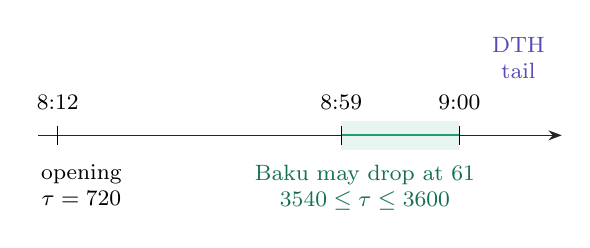
\begin{tikzpicture}[x=1cm,y=1cm,every node/.style={font=\footnotesize}]
\draw[-{Stealth},figink] (0.25,0)--(6.9,0);
\fill[figpaleteal] (4.1,-0.18) rectangle (5.6,0.18);
\draw[figteal,thick] (4.1,0)--(5.6,0);
\foreach \x/\label in {0.5/{8:12},4.1/{8:59},5.6/{9:00}} {
  \draw (\x,-0.12)--(\x,0.12);
  \node[anchor=south] at (\x,0.2) {\label};
}
\node[anchor=north,align=center] at (0.8,-0.25) {opening\\$\tau=720$};
\node[anchor=north,align=center,text=figteal!70!black] at (4.4,-0.25) {Baku may drop at 61\\$3540\le\tau\le3600$};
\node[anchor=south,align=center,text=figpurple] at (6.35,0.6) {DTH\\tail};
\end{tikzpicture}
\figcap{Baku can drop at 61 in the leap window. After 9:00, both players use seconds 1 to 60. The timeline is schematic.}
\vspace{12pt}
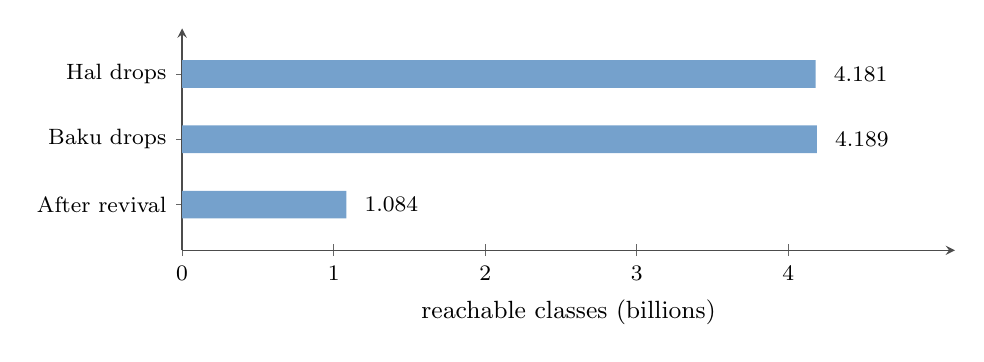
\begin{tikzpicture}
\begin{axis}[
 width=0.94\linewidth,height=4.4cm,xbar,
 xmin=0,xmax=5.1,ytick={1,2,3},
 yticklabels={After revival,Baku drops,Hal drops},
 y dir=normal,bar width=10pt,
 xlabel={reachable classes (billions)},
 xtick={0,1,2,3,4},axis lines=left,
 enlarge y limits=0.35,nodes near coords,
 nodes near coords align={horizontal},
 nodes near coords style={font=\footnotesize,anchor=west,xshift=3pt},
 point meta=explicit symbolic,
]
\addplot[fill=figblue!65,draw=none] coordinates {
 (1.084020312,1) [1.084]
 (4.188677815,2) [4.189]
 (4.180634990,3) [4.181]
};
\end{axis}
\end{tikzpicture}
\figcap{We count each reachable quotient state once. The revival group contains Baku's turns after he survives an injection.}
\raggedright
\head{3. The extra second}
We use the DTH payoff matrix $M$ [1, Section 4], with success
payoffs $S_\ell$ and failure payoff $F$. The value $V$ is the current
Dropper's win probability minus loss probability; a role swap negates it.
We evaluate the continuation states at their new clocks.

Successes share one child clock; failures share another for the given
Checker profile. We still need only 60 success payoffs and $F$.
In Baku's window, we add a row of 60 copies of $F$.
If $v_{60}$ is the square matrix value, then
\[
\boxed{v_{61}=\max\{v_{60},F\}.}
\]
\textbf{Proof.} Give the extra row mass $\alpha$ and an ordinary
Dropper mixture $a$ the remaining mass. The guaranteed payoff is
$\alpha F+(1-\alpha)\min_c(a^{\mathsf T}M)_c$.
We maximize over $a$, then choose the better endpoint in $\alpha$.
The Checker can use a minimizing mixture for $M$ in either case.
\textup{QED}
\end{minipage}
\newpage
\begin{minipage}[t]{0.55\textwidth}
\vspace{0pt}
\head{4. Solving the round}
We use the fixed-action test and mixed-strategy recurrence from
DTH [1, Section 4]. We check each candidate against the same
$10^{-6}$ saddle-gap limit. The extra second changes the continuation
values, and some states need linear programming to meet this limit.

\head{5. Linear programming}
For an unresolved stage with $\delta=F-S_1>0$, define
\[
A_{ij}=\begin{cases}(F-S_{j-i+1})/\delta,&j\ge i,\\0,&j<i.\end{cases}
\]
Then $M=F\mathbf1\mathbf1^{\mathsf T}-\delta A$, with unit diagonal
in $A$. We solve the dual linear programs
\[
\max_{y\ge0}\{\mathbf1^{\mathsf T}y:A^{\mathsf T}y\le\mathbf1\}
=\min_{z\ge0}\{\mathbf1^{\mathsf T}z:Az\ge\mathbf1\}=Z.
\]
\textbf{Proof.} The unit diagonal gives a finite nonnegative covering
vector by back substitution; zero is feasible for packing.
Linear-programming duality gives a common optimum $Z>0$.
For $a=y/Z$ and $b=z/Z$, we obtain
$a^{\mathsf T}M\ge(F-\delta/Z)\mathbf1^{\mathsf T}$ and
$Mb\le(F-\delta/Z)\mathbf1$. Thus $v_{60}=F-\delta/Z$.
\textup{QED}

We solve the remaining stages by linear programming. For a candidate
Dropper mixture $a$ and Checker mixture $b$, we bound the value with
\[
L=\min_c(a^{\mathsf T}M)_c,\qquad U=\max_d(Mb)_d.
\]
In the leap window, we replace each bound by its maximum with $F$.
We require $U-L\le10^{-6}$ and use the midpoint or a center with
proved error at most $5\times10^{-7}$.

\head{6. Error bounds}
We retain the DTH progress score $\Phi$ and its bound of 1,201 steps
[1, Sections 3 and 5]. The clock adds no cycles, and the extra
failure row uses the same injection transition. Thus the DTH error
proof also covers this extension:
\[
|\widehat V-V|\le(1201-\Phi)5\times10^{-7}.
\]
At the opening, the win-probability error is at most $0.000301$.
We use floating-point saddle checks for the matrix and LP paths.
We re-solve 4,621 sampled stages by linear programming. The largest
difference from the stored values is $3.07\times10^{-9}$.

\end{minipage}\hfill
\begin{minipage}[t]{0.42\textwidth}
\vspace{0pt}
\centering
\includegraphics[width=\linewidth]{build/figures/stl/strategy_surface.pdf}
\figcap{Hal's drop strategy at 16 reachable states, one per minute from
8:44 to 8:59. Hal has $(s,t)=(0,180)$; Baku has $(60,120)$.
We hold these profiles fixed and join adjacent clock slices.
Each slice is a separate state. Hal puts $95.77\%$ on second 1
at 8:50 and $41.31\%$ at 8:51.}
\vspace{5pt}
\raggedright
\setlength{\parskip}{4pt}
\head{7. Results}
At the starting state, we obtain
\[
\begin{gathered}
V=0.03717\pm0.00061,\\
P(\text{Hal wins})=0.51859\pm0.00031.
\end{gathered}
\]
We solve 8,843,634,465 classes with fixed actions or the recurrence
and gap check, and 609,698,652 with linear programming.

Baku wins $48.14\%$ of games, a gain of $2.63$ percentage points
over the base game. Hal's win probability falls from $54.49\%$ to
$51.86\%$. A successful check and a survived injection lead to
different clocks. The players must account for who will drop when
the extra second arrives, so their strategies can change before
the leap window even at fixed loads (Figure 3).

{\footnotesize\textbf{References.} [1] J. Cenawood,
\href{dth_exact_solution.pdf}{\emph{Solving Drop the Handkerchief}},
September 11, 2026.
[2] NICT, \href{https://www.nict.go.jp/en/sts/jst.html}{\emph{Japan Standard Time}};
\href{https://www.nict.go.jp/publication/NICT-News/0810/09.html}{leap-second notice},
October 2008.
[3] T. Sako, \emph{Usogui}, Shueisha, 2006--2018.}
\end{minipage}
\end{document}
